\documentclass[conference]{IEEEtran}
\usepackage{graphicx}
\begin{document}

\title{Twitter Topic Summarization using Speech Acts and Sequential Summarization}
\author{
\IEEEauthorblockN{Under the guidance of}
\IEEEauthorblockA{Dr. A. P. Shanthi \\ Associate Proffesor \\ Department of Computer Science and Engineering \\ College of Engineering Guindy\\ Anna University}
\and
\IEEEauthorblockN{Submitted By}
\IEEEauthorblockA{Daniel Sam Pete, Dinesh, Gopinathan \\ Computer Science and Engineering\\
College of Engineering Guindy\\ Anna University}
}

\maketitle
\begin{abstract}

\par In a micro-blog such as twitter there is a wide array of tweets on each topic of interest according to the user. The tweets are noisy, conversations, express opinions and suggestions and may notify of a change of events in the current trend.

\par In order to enable users to quickly view a summary about a topic searched, a system is proposed in which given an input query topic, the best relevant tweets are retrieved by the system using speech act recognition which is a multiclass classification problem solved using the word based linguistic features and features based on twitter. The unwanted tweets are ignored and then an abstract summary is formed. Summarization is done based on stream-based and semantic-based. Stream based is that a collection of tweets are collected and are split up into different sets based on the timing of the tweet. Due to some hindrances a tweet on a sub topic may be put up in different set of tweets and so a semantic-based subtopic detection and summarization is necessary. After finding out the subtopics, measure of Local Relevance, Global relevance and crowding endorsement are also found out to enhance the summarizer.

\end{abstract}

\maketitle
\begin{keywords}
Machine Leaning, Natural Language Processing
\end{keywords}

\IEEEpeerreviewmaketitle
\section{\textbf{Problem Statement}}

\par To build a system that helps to get a topic oriented summarization from tweets and gains information from them. In this system we plan on using basic speech acts like question, suggestion, comment, suggestion, miscellaneous  to find the tweets containing information and using relevance between the tweets to minimize the redundant information.

\section{\textbf{Applications}}

\par It could be used to generate abstractive summaries for news articles, technical articles, and briefings. It could be used to find the general opinion of People which would help the world in a variety of ways.

\section{\textbf{Literature Review}}

\subsection{\textbf{Automatic Twitter Topic Summarization With Speech Acts [Renxian Zhang, Wenjie Li, Dehong Gao, and You Ouyang]}}

\par This paper proposes a speech act-based approach to Twitter topic summarization. The approach to topic summarization is employed in three Core modules: recognizing speech acts in tweets(using an SVM based on linguistic word features and features because of twitter), extracting speech act-guided key words/phrases(finding out the important key words/phrases based on speech acts) and generating abstractive summaries by generating a score based on hash topic information and also creation of templates for each of the speech acts and deriving the ngrams from the tweet for the template.

\subsection{\textbf{Sequential Summarization: a Full View of Twitter Trending Topics [Dehong Gao, Wenjie Li, Xiaoyan Cai, Renxian Zhang and You Ouyang]}}

\par Sequential summarization, which aims to provide a serially  ordered short sub-summaries for a trending topic in order to provide a complete story about the development of the topic while retaining the order of information presentation. Two approaches i.e., stream-based and semantic-based approaches are developed to detect the important subtopics within a trending topic. Stream based approach is done by splitting up tweets into different sets based on time surges. Semantic based sub topic detection is done because a sub topic can also be distributed into different sets.Thus measures of Local Relevance, Global relevance, Crowding Endorsements are included. In addition,it proposes three new measures to evaluate the position-aware coverage, sequential novelty and sequence correlation of the system-generated summaries. Then a short sub-summary is generated for each subtopic.

\subsection{\textbf{Comparing Twitter Summarization Algorithms for Multiple Post Summaries [David Inouye* and Jugal K. Kalita+]}}

\par In this paper, a Frequency based summarizer (involving Sum Basic and Hybrid TF-IDF) was proved to provide better results than the other 6 summarizer’s used. Eight different summarizers: random, most recent, MEAD, TextRank, LexRank, cluster, Hybrid TF-IDF and SumBasic. A threshold was used to find out similarity.

\subsection{\textbf{TweetMotif: Exploratory Search and Topic Summarization for Twitter [Brendan O’Connor, Michel Krieger,David Ahn]}}

\par In this paper, TweetMotif Search application groups messages by statistically unlikely phrases that co-occur the themes of the conversation. Also the text analysis system also clusters near duplicates and uses other techniques to improve your view of the twitter lands. TweetMotif to deflate rumors, uncover scams, summarize sentiment, and track political protests in real-time.

\subsection{\textbf{Summarizing Microblogs Automatically [Beaux Sharifi, Mark-Anthony Hutton and Jugal Kalita]}}

\par A short one line summary of a topic based on all the tweets that are related to that topic based on a PR(Phrase Reinforcement)algorithm. First the most talked about topic is found using the most occurring phrase or word and it can also be found based on retweet count. After finding out the phrase they filter out spam or irrelevant data. After that a graph is formed and PR algorithm is used to form a one line summarizer.

\subsection{\textbf{Multiple Post Microblog Summarization[David Inouye]}}

\par In this paper they have first clustered the tweets using clustering algorithms like k means, k bisecting means algorithms and have clustered tweets based on sub topics and in these cluster of sub topics a sub summary is developed using various summarization algorithms like hybrid TF-IDF algorithm.

\subsection{\textbf{What Are Tweeters Doing: Recognizing Speech Acts in Twitter[Renxian Zhang; Dehong Gao; Wenjie Li]}}

\par This paper does multi class classification of the various speech acts in twitter. It involves design of a feature set based on cue words and phrases, non cue words, character based and annotation based. The training data was taken based on topic level, the whole twitter dataset and category level.

\section{\textbf{Specifications}}
\subsection{\textbf{Hardware Requirements(Minimum)}}
\begin{enumerate}
\item{256 RAM}
\item{30 MB free Hard Disk Space}
\item{Intel Pentium/AMD Processor}
\end{enumerate}

\subsection{\textbf{Software Requirements}}
\begin{itemize}
\item{Win XP/7/8}
\item{OCTAVE for Windows}
\item{Java/Phyton}
\end{itemize}

\section{\textbf{Block Diagram}}
\begin{center}
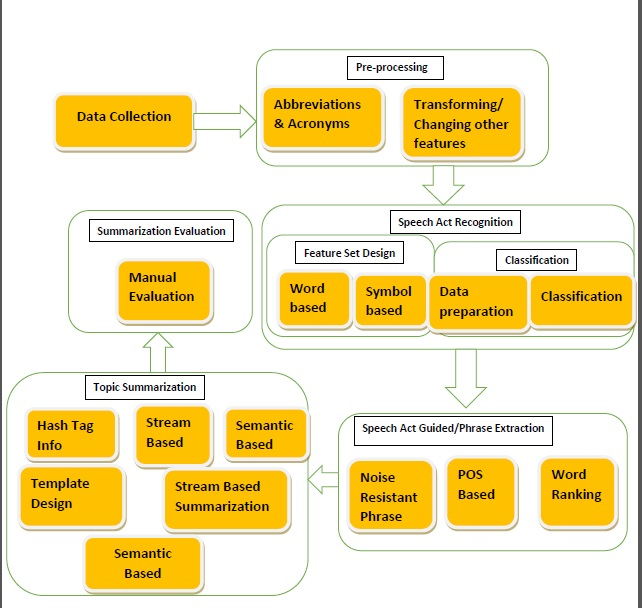
\includegraphics[scale=0.5]{module.jpg}
\end{center}

\section{\textbf{System Design}}
\subsection{\textbf{Data Collection}}
\par Using Twitter Api to get the tweets which are used for our Topic Summarization.

\subsection{\textbf{Preprocessing}}

\subsubsection{\textbf{Abbreviations and acronyms}}

\par A module in which abbreviation of all acronyms which are used in social networking sites like im, 4ever etc is done.

\subsubsection{\textbf{Transforming/Changing other features}}

\par A module in which all words are translated into lower cases for better results,email addresses and urls are removed and tagged. Emoticons are looked up with the database and we find out the sentiment with which the tweet was delivered if possible. Unwanted characters are removed(excess of fullstops).

\subsection{\textbf{Speech act Recognition}}

\begin{enumerate}
\item{\textbf{Feature Set Design}}
A module in which all the features which are required to classify between the different speech acts.

\subsubsection{\textbf{Word based features}}
\textbf{CUE WORD}

\par Using a linguistic word based feature set, for eg “whether”  would mostly signify that the sentence is a question and “could you please” would mostly signify a suggestion. So a list of specific unigrams, bigrams and trigrams are found out which would enhance the classifier.

\par In addition to this, if the sentence is properly formed, the sentence would be pos tagged and depending on specific grammatical rules which is highly likely would also help to enhance the classifier.
		
\par \textbf{NON CUE WORD}
\par Feature set based on the abbreviations and acronyms commonly used on the internet like “tq”, ”4ever” etc. Opinion words collected from sentiwordnet. Emoticons could signify the amount of Emotion into the tweet and the postive or negativity of the tweet which could be found out by sentiwordnet. They could also be taken into account for the classification of Sentences. Vulgar word which could be found out with a straight forward word check. These could enhance the classifiers ability to classify correctly.

\begin{table}[!ht]
\centering

    \label{tab:Cue Words and Phrases}

    \begin{small}
    \begin{tabular}{|p{1.5cm}|p{4cm}|}
    \hline {\bfseries Input} & {\bfseries Examples} \\
    \hline
     Unigrams &  know, hurray, omg, why, pls..\\
     \hline
     Bigrams & do it, i bet, you can, ima need.. \\
     \hline
     Trigrams & ?!?, heart goes out, rt if you..\\
     \hline
    \end{tabular}
    \end{small} 
\end{table}

\subsubsection{\textbf{Symbol based features}}
\par “?” mostly signifies that the tweet is a question and it could also signify a confused state .  ”!” Could signify an exclamatory sentence or an excited state.Twitter Specific symbols are RT(Retweet),@(directed towards a person through acts of dialogue),\#(denotes a topic or comment). A RT strongly indicates the presence of a statement.

\subsection{\textbf{Classifier}}

\subsubsection{\textbf{Training Phase}}
\par With the help of annotated data the system is trained which will be helpful in classification of unclassified tweets.

\subsubsection{\textbf{Feature Extraction and Classification Phase}}
\par The commonly used bag of words feature set is used and features are extracted from the unclassified tweet and it is classified using \textbf{SVM}.

\subsubsection{\textbf{Speech Act types and Other speech act types and Examples}}
\begin{table}[!ht]
\centering

    \label{tab:Speech Act Types}

    \begin{small}
    \begin{tabular}{|p{1.5cm}|p{1.8cm}|p{4cm}|}
    \hline {\bfseries Searle's types} & {\bfseries Our Types} &{\bfseries Example Tweets} \\
    \hline
     Assertive &  Statement & Libya Releases 4 Times Journalists http://www.photozz.com/?104k\\
     \hline
     Directive & Question & #sincewebeinghonest why u so obsessed with what me n her do?? Don’t u got ya own man??? Oh wait… \\
     \hline
     Directive & Suggestion & RT @NaonkaMixon: I will donate 10 \$ to the Red Cross Japen EarthQuake fund for every person that retweet this! #PRAYFORJAPAN \\
     \hline
     Expressive & Comment & is enjoying this new season of #CelebrityApprentice… Nikki Taylor=Yum!! \\
     \hline
     Commissive and declarative & Miscellaneous & 65. I want to get married to someone I meet in highschool. #100factsaboutme \\
     \hline
    \end{tabular}
    \end{small} 
\end{table}


\item{\textbf{Classification Evaluation}}
\end{enumerate}

\begin{itemize}

\item{\textbf{Data Preparation}}
\par A suitable data set for a supervised classification algorithm is used.

\item{\textbf{Classification}}
\par A module in which tweets are classified in each topic using different feature sets employing SVM algorithm  using a linear kernel or logistic regression. A cross validation is done and a feature set is mixed up and used to see which feature set is the best and removal of redundant  features. An F1 score can be computed to find out the correctness of the classifier and and cross fold validations can also be done.
\end{itemize}

\subsection{\textbf{Speech act guided keyword/phrase extraction}}
\subsubsection{\textbf{Noise Resistant Phrase Extraction}}
\par In this module we try to extract key words and phrases from the tweets of major speech act types after removing stop words. A list of stop words are collected from an online resource. Then all the less informative words are removed and n grams are extracted. Likelihood of the n grams are found using two hypotheses H0 and H1, where H0 denotes occurrences of n grams are independent and H1 denotes occurrence of n grams are dependent and calculate \log(H0)/\log(H1). 

\par Likelihoods are calculated using n-nomial distribution and n gram probabilities are calculated using \textbf{Maximum Likelihood Estimation Algorithm}.

\par Extracting the key phrases is formulated as finding frequent n-gram collocations. The topmost number of bigrams and trigrams are extracted and utilised.

\subsubsection{\textbf{POS based Phrase Extraction}}
\par Statements are about facts, things, people, etc. and suggestions are about actions, activities, etc. Such information can be approximated by part-of-speech (POS) patterns for both words and phrases.
 \par The statement-relevant word is a noun, or ‘/N/’, phrase is a noun phrase, such as ‘/Adj/ /N/’(e.g., high quality) and ‘/Adj/ /N/ /N/’ (e.g., sexual abuse charges).
\begin{itemize}
\item{The comment-relevant POS patterns are like the statement relevant
Ones. But they must have at least one opinion word (e.g., good thing) judged from SentiWordNet and the compilation of words.}
\item{The suggestion-relevant word is a verb, or ‘/V/’ (e.g., hate), phrase is verb-centered10, such as ‘/Adv/ /V/’ (e.g., truly wish) and ‘/V/ /N/ /N/’ (e.g., sell health drugs).}
\item{The question-relevant word is either a verb or a noun, or (/‘N’/ /‘V’/) (e.g.,reason), phrase is either a noun phrase or a verb-centred phrase, such as ‘/Adj/ /N/ /N/’ (e.g., dirty ass mirror).}
\end{itemize}

\subsubsection{\textbf{Phrase/Word Ranking}}
\par A graph for the tweets of a major speech act type, using the extracted ngrams (Ng) as vertices. Two vertices and are linked by an edge if they co-occur in some tweet and the weight of the edge is the number of such co-occurrences. Then we define a graph score which is a formula and with the help of it we can find out the more important phrases, which would be useful for summarising.

\subsection{\textbf{Topic Summarization}}
\subsubsection{\textbf{Hash tag info}}
\par Use hash tag for information related to the topic by splitting it up.

\begin{center}
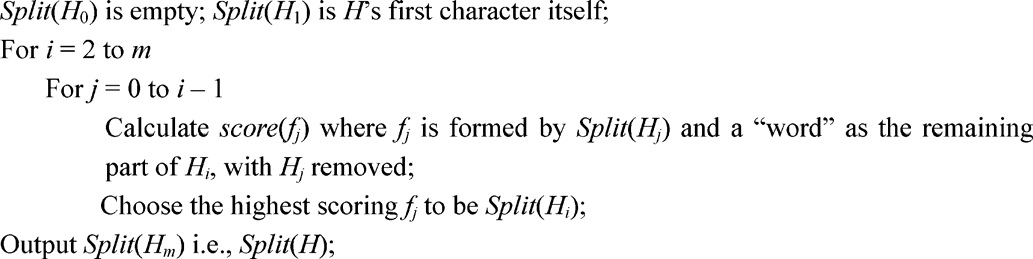
\includegraphics[scale=0.3]{hashtag.jpg}
\end{center}

\subsubsection{\textbf{Stream-based subtopic detection}}
\par The stream-based subtopic detection then is to identify these peak areas from the tweet stream about a specific topic. The Offline Peak Area Detection (OPAD) algorithm used in the reference paper [2], to locate peak areas by tracing the volume changes of tweet streams. The subtopic detection can be formalized as: given the tweet stream, detect a serial of peak areas, a set of tweets and denote the start and end time point of the peak area respectively. We use the tweets in the surges to represent the subtopics.

\begin{center}
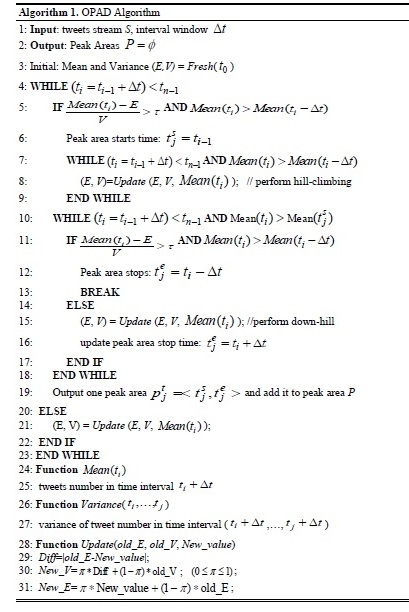
\includegraphics[scale=0.80]{OPAD1.jpg}
\end{center}


\subsubsection{\textbf{Semantic-based subtopic detection}}
\par To identify subtopics from the semantic perspective, Stream-based subtopic detection utilizes the volume change of the tweet stream to identify the subtopics. However, as mentioned before, due to the differences of geographical and time zones, Twitter may collect tweets about a same subtopic at different times. As a result, a subtopic may be separated into different peak areas or a peak area may contain a mix of more than one subtopic. To identify subtopics from the semantic perspective, semantic-based subtopic detection is proposed to employ Dynamic Topic Model to capture subtopics in the tweet stream.

\par DTM regards the topics evolve over time and supposes that the data is divided by a special time interval. The tweets in each time interval are modelled by K-component topic model, and the subtopic associated with the time interval t evolves from the subtopic associated with the time interval t-1.

\subsubsection{\textbf{Template Design}}
\par Insert the information so far gathered and putting them in slots of a basic template.

\subsubsection{\textbf{Stream based sequential summarization algorithm}}
\par A summarization algorithm is used to summarize all the sentences so far extracted from the text based on local relevance, global relevance and crowd endorsement by using a cosine similarity formula.

\par The global relevance of the tweet $s_i$ is defined as the cosine similarity between the tweet $s_i$ and the entire stream S, 

\begin{center}
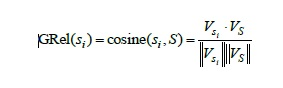
\includegraphics[scale=0.8]{formula1.jpg}
\end{center}

\par \textbf{Local Relevance:} Assume that the tweets in a peak area represent a subtopic in the topic. The local relevance of the tweet $s_i$ is defined as the cosine similarity between the tweet $s_i$ and the tweets in the peak area that belongs to, i.e.$p_j$

\begin{center}
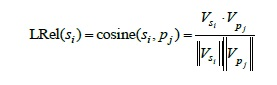
\includegraphics{formula2.jpg}
\end{center}

\par \textbf{Crowding Endorsement:} The endorsement of the tweet $s_i$ from the crowds is measured by the normalized re-tweeting count.

\begin{center}
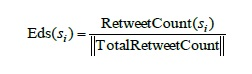
\includegraphics{formula3.jpg}
\end{center}

\subsubsection{\textbf{Semantic based summarization algorithm}}
\par We use the output probabilistic relationships between tweets and subtopics to assign each tweet to the subtopic that it most likely belongs to. Then the subtopics are ordered by the mean timestamp of the tweets in the corresponding subtopics. A score is computed for each sentence from the corpus collected and selected .Then the tweets with the highest scores are selected for each subtopic. MMR (Minimum of Minimum Roughness) or a k-means clustering algorithm is used to remove redundancy in the generation of each sub-summary in both cases. For each tweet to be selected into sub-summary, it is compared against the tweets that are already selected in the previous sub-summaries. The tweet is selected only when it is considered not significantly overlapping any previously selected tweets.  Similarity measurements and novelty measurements used in [11] are used to find similarity.

\section{\textbf{Description of how the final work will be displayed}}
\par An input BJP given to the summariser should summarise all the tweets collected so far based on the types of speech acts and keyword extraction techniques some of the tweets will be neglected for summarisation. The informative ones will be used for summarisation. A short sequential summary will be displayed on the computer.

\section{\textbf{Final Work to be done}}
Given a topic a user should view an abstract summary of the Topic.

\subsection{\textbf{Input:} BJP}
RT @IBNLivePolitics: Delhi: Hit by Vijay Goel's rebellion, BJP defers naming CM candidate http://ibnlive.in.com/news/delhi-hit-by-vijay-goels-rebellion-bjp-defers-naming-cm-candidate/429510-37-64.html …

BJP releases list of candidates for Chhattisgarh assembly elections http://www.ndtv.com/article/assembly-polls/bjp-releases-list-of-candidates-for-chhattisgarh-assembly-elections-434814 …

BJP's Delhi CM candidate: Vijay Goel stakes claim  http://dnai.in/bLFy  pic.twitter.com/duLtIGde4C

Delhi BJP's Vijay Goel threatens to quit if not made chief ministerial candidate

News Flash: Delhi BJP president Vijay Goel storms out of meet held to take a  decision on the party's Delhi CM candidate

\subsection{\textbf{Output}}
Delhi BJP President Vijay Goel storms out of meet held to take a decision on the party’s Delhi Chief Ministerial candidate. Hit by his rebellion BJP defer naming Chief Ministerial candidate. He threatens to quit if not made Chief ministerial candidate.

\section{\textbf{Module Input/Output}}
\subsection{\textbf{Data Collection}}

\subsubsection{\textbf{Input:} A Keyword}
BJP

\subsubsection{\textbf{Process}}
\par A twitter API call is made and the tweets are retrieved

\subsubsection{\textbf{Output:} A Set of Tweets}
\begin{enumerate}
\item{subtlechat There will always be issues between AAP and Congress Live-in. Only AAP and BJP can form a ideologically similar relationship for long term. }

\item{LakshminarayanK @mylovenamo @DhrumilBJP It will be fantastic if this can really be achieved by BJP in every constituency.}

\end{enumerate}

\subsection{\textbf{Preprocessing}}

\subsubsection{\textbf{Input}}
Tweets
\subsubsection{\textbf{Process}}
\par A simple look up of a lexicon of words.

\subsubsection{\textbf{Output}}
Expanded Set of Tweets: vivek joshy RT @narendramodi: Thank you for that Mr.Modi  \# BJP

\subsection{\textbf{Transforming/Changing}}

\subsubsection{\textbf{Input}}
Tweets
\begin{enumerate}
\item{askkaushik @PritishNandy if congress back off now, it will prove that they r scared of AAP. They would be safer with BJP in power.}
\item{vivek joshy RT @narendramodi: Attended Party meetings in Delhi today http://t.co/H1WqdKOk2B}
\end{enumerate}

\subsubsection{\textbf{Process}}
\par A module in which cases are transformed, urls, mail id’s, hash topics are tagged and excessive punctuation is removed and compression of words like hiiiiiiiiiiiii to hi.

\subsubsection{\textbf{Output}}
\par A set of compression and expansion of certain words in tweets and tagged tweets.
\begin{enumerate}
\item{$<$user$>$ $<$directed at$>$ if congress back off now, it will prove that they are scared of aap. They would be safer with bjp in power.}
\item{$<$user$>$ rt $<$directed$>$ at attended party meetings in delhi today URL}
\end{enumerate}

\subsection{\textbf{Speech Act Recognition}}
\subsubsection{\textbf{Input}}
Preprocessed Tweets
\begin{enumerate}
\item{$<$user$>$ rt $<$directed at$>$ attended party meetings in delhi today $<$URL$>$ }
\item{$<$user$>$ bjp's jaitley says whole of india `disillusioned' - bloomberg for ipad $<$url$>$}
\end{enumerate}
\subsubsection{\textbf{Process}}
\par An annotated data set for training the SVM and using a SVM classifier with a linear kernel is used for classification is done using a bag of words feature set.

\subsubsection{\textbf{Output}}
Classified Set of Tweets
\begin{enumerate}
\item{$<$user$>$ rt $<$directed at$>$ attended party meetings in delhi today $<$URL$>$ -Statement}
\item{$<$user$>$ bjp's jaitley says whole of india `disillusioned' - bloomberg for ipad $<$url$>$-Comment}
\end{enumerate}

\subsection{\textbf{Speech act guided Key word extraction}}
\subsubsection{\textbf{Input}}
Classified Set of Tweets
\begin{enumerate}
\item{Comment
$<$user$>$ There will always be issues between AAP and Congress Live-in. Only AAP and BJP can form a ideologically similar relationship for long term.}
\item{Comment
$<$user$>$$<$directed at$>$$<$directed at$>$ It will be fantastic if this can really be achieved by BJP in every constituency. }
\item{Statement
$<$user$>$ RT $<$directed at$>$ BJP targets 272+ seats on own, plans Modi for PM fund(Video) $<$url$>$ }
\item{Miscellaneous
$<$user$>$ RT $<$directed at$>$ CBI giving a clean chit to Amit Shah doesn't mean that he is innocent. All it means is that CBI now believes BJP will come}
\item{Comment
$<$user$>$ $<$directed at$>$ if congress back off now, it will prove that they r scared of AAP. They would be safer with BJP in power}
\item{Miscellaneous
$<$user$>$ RT $<$directed at$>$: Don't know if AAP is falling into Congress trap,or Congress is falling in AAP trap.But thank god BJP is not falling in either.}
\item{Statement
$<$user$>$ RT $<$directed at$>$ Attended Party meetings in Delhi today $<$url$>$ }
\item{Comment
$<$user$>$ BJP's Jaitley Says Whole of India `Disillusioned' - Bloomberg for iPad $<$url$>$}
\item{Statement
$<$user$>$ RT $<$directed at$>$ Attended Party meetings in Delhi today $<$url$>$}

\end{enumerate}
\subsection{\textbf{Noise Resistant Phrase Extraction}}
\subsubsection{\textbf{Process}}
\par An n-gram extraction algorithm which extracts an n-gram from the tweet for information.
\subsubsection{\textbf{Output}}
Phrases of information gathered from tweets
\begin{enumerate}
\item{issues between AAP and Congress Live-in,  AAP and BJP form  ideologically similar relationship long term}
\item{BJP achieved constituency}
\item{BJP target 272+ seats, Modi, PM fund}
\item{CBI chit Amit Shah ,innocent, BJP, CBI }
\item{Congress back off, AAP scared}
\item{AAP ,Congress,  trap Congress, AAP  trap BJP}
\item{Party Meetings, Delhi}
\item{Jaitley ,Whole of India Disillusioned ,Bloomberg of Ipad}
\item{Party Meetings, Delhi}
\end{enumerate}

\subsection{POS guided Key word extraction}
\subsubsection{\textbf{Process}}
Based on the speech act the important key set of information is extracted.

\subsubsection{\textbf{Output}}
Key words extracted from tweets
\begin{enumerate}
\item{Comment
issues between AAP and Congress Live-in. AAP and BJP can form a ideologically similar relationship for long term.}
\item{Comment
achieved by BJP in every constituency}
\item{Statement
272+ seats on own, Modi for PM fund (Video)}
\item{Comment
 safer with BJP in power}
 \item{Statement
 Party meetings in Delhi today}
 \item{Comment
Whole of India `Disillusioned'}
\item{Statement
Party meetings in Delhi today}
\end{enumerate}

\subsection{\textbf{Phrase Word Ranking}}
\subsubsection{\textbf{Input}}
Set of phrases, keywords from tweets

\subsubsection{\textbf{Process}}
Graph is formed and a score is calculated based on edge weight with vertices as phrases and edges formed based on co-occurrence in tweets.

\subsubsection{\textbf{Output}}
A score for each of the phrases

\subsection{\textbf{Summarizer}}
\textbf{Hash Topic}
\subsubsection{\textbf{Input}}
Tweets with hash tag \# ihatebjp

\subsubsection{\textbf{Process}}
An algorithm with which the topic is split up correctly.

\subsubsection{\textbf{Output}}
Correct split up of tweets: i hate bjp.

\subsubsection{\textbf{Input for remaining modules}}
Timestamped Tweets
\begin{enumerate}
\item{Comment\\$<$Timestamp 1$>$
issues between AAP and Congress Live-in. AAP and BJP can form a ideologically similar relationship for long term.}
\item{Comment\\$<$Timestamp 2$>$
It will be fantastic if this can really be achieved by BJP in every constituency. }
\item{Statement\\$<$Timestamp 3$>$
BJP targets 272+ seats on own, plans Modi for PM fund (Video)}
\item{Comment\\$<$Timestamp 4$>$
 congress back off now,  prove that they r scared of AAP.  safer with BJP in power}
 \item{Statement\\$<$Timestamp 5$>$
 Party meetings in Delhi today}
\item{Comment\\$<$Timestamp 6$>$
Whole of India `Disillusioned' }
\item{Statement\\$<$Timestamp 7$>$
Party meetings in Delhi today}
\end{enumerate}


\subsection{\textbf{Stream Based Subtopic Detection}}
\subsubsection{\textbf{Process}}
\par Based on OPAD and using peak area concept, the set of peaks are extracted and the set of subtopics are found out.

\subsubsection{\textbf{Output}}
Subtopics and tweets related to them.

\subsubsection{\textbf{Local Peak}}
\textbf{Subtopic:} Party Meetings(in timestamps 5 and 7)\\
5) Statement
Party meetings in Delhi today \\
7) Statement
Party meetings in Delhi today.

\subsection{\textbf{Semantic Based Subtopic Detection}}
\subsubsection{\textbf{Process}}
\par Dynamic Topic Modelling is used to get sub topics and their tweets. From DTM, we can obtain two distributions, the topic distribution of the tweets and the word distribution of topics.

\subsubsection{\textbf{Output}}
Set of k subtopics and tweets in those topics.

\subsubsection{\textbf{Subtopic}}
\textbf{AAP}
issues between AAP and Congress Live-in. AAP and BJP can form a ideologically similar relationship for long term \\
congress back off now,  prove that they r scared of AAP. safer with BJP in power. 

\subsection{\textbf{Templates}}
\subsubsection{\textbf{Input}}
Keywords from tweets, classified tweets.\\
Suggest, do your job.
\subsubsection{\textbf{Process}}
Based on the speech act, the correct template is used.

\subsubsection{\textbf{Output}}
Templated sentences.\\
The suggestion is to do your job.

\subsection{\textbf{Ranking of tweets and summary}}
\subsubsection{\textbf{Process}}
\par Removal of redundancy using k means clustering or MMR. A summary is formed from k components got out from the DTM. For each kth sub topic, the score is calculated for each tweet using the formula in [2] and the tweets with maximum score is incorporated into the summary.

\subsubsection{\textbf{Output}}
A summary of tweets.\\
\par The general opinion among people is that there will always be issues between AAP and Congress, though BJP can form an ideologically similar relationship with AAP. It is of the general opinion that if congress back off now then it’ll prove they are afraid of AAP. BJP targets 272+ seats on own, plans Modi for PM fund BJP Party Meetings held in Delhi today.





\section{\textbf{Validation}}

\subsection{\textbf{Manual Checking}}
The summaries generated are manually checked for correctness.

\subsection{\textbf{Evaluation of Sub topic detection}}
\par A manual check up is infeasible, an automated check up of similar sub topics can be done by finding out cosine similarity.

\subsection{\textbf{Classifiction Evaluation}}

\subsubsection{\textbf{Preparation}}
A suitable data set for a supervised classification algorithm is used.

\subsubsection{\textbf{Classification}}
\par A module in which tweets are classified in each topic using different feature sets employing SVM algorithm using a linear kernel or logistic regression. A cross validation is done and a feature set is mixed up and used to see which feature set is the best and removal of redundant features. An F1 score can be computed to find out the correctness of the classifier and cross fold validations can also be done.

\section{\textbf{Tools Used}}

\begin{enumerate}
\item{Octave}
\item{Standard POS Tagger}
\item{Twitter API}
\item{Python/Java}
\end{enumerate}
 \par \textbf{OCTAVE (Operationally Critical Threat, Asset, and Vulnerability Evaluation)} is a suite of tools, techniques, and methods for risk-based information security strategic assessment and planning. Since it is easy to use it in Matrix, It is easy to employ Machine Learning algorithms.

\section{\textbf{Datasets}}
\par A set of annotated data sets are available online.
www4.comp.polyu.edu.hk/~csrzhang/files/Public.
A set of Swearing words
http://www.noswearing.com/dictionary.
A list of Emoticons used in the Internet
http://www.sharpened.net/emoticons/.
Chat Language and their Interpretation
http://www.chatslang.com
 
 \par The annotated data set is used for training to enhance the classification of speech acts. The set of swearing words are used to find out the abusive/unwanted words used in the tweets and use it to our advantage during classification. The list of Emoticons and their interpretation is used for finding out the intent/emotion of the user tweeting. The chat slang dataset is the most important one. Because of the modern age of chatting the language of chat is a dictionary in itself and so we need to know the usage of certain words for which this would be helpful.


\begin{thebibliography}{1}

  \bibitem{IEEEhowto:zhang}
  Renxian Zhang, Wenjie Li, Dehong Gao and You Ouyang, \emph{Automatic Twitter Topic Summarization With Speech Acts} Audio, Speech, and Language Processing, IEEE Transactions on  Volume:21,  Issue: 3, March 2013. 

\bibitem{IEEEhowto:gao}
Dehong Gao, Wenjie Li, Xiaoyan Cai, Renxian Zhang and You Ouyang, \emph{Sequential Summarization: a Full View of Twitter Trending Topics} Audio, Speech, and Language Processing, IEEE Transactions on  Volume: PP,  Issue: 99, September 2013. 
\bibitem{IEEEhowto:inouye}
David Inouye* and Jugal K. Kalita+, \emph{Comparing Twitter Summarization Algorithms for Multiple Post Summaries} Privacy, security, risk and trust (passat), 2011 ieee third international conference on and 2011 IEEE third international conference on social computing (socialcom), October 2011.
\bibitem{IEEEhowto:brendan}
Brendan O’Connor, Michel Krieger,David Ahn, \emph{TweetMotif: Exploratory Search and Topic Summarization for Twitter} 2010.
\bibitem{IEEEhowto:beaux}
Beaux Sharifi, Mark-Anthony Hutton and Jugal Kalita, \emph{Automatic Summarization of Twitter Topics} University of Colorado at Colorado Springs, 2010
\bibitem{IEEEhowto:sharfi}
B.Sharifi, M.-A. Hutton, and J. Kalita,  \emph{Experiments in microblog summarization} in Proc. IEEE 2nd Int. Conf. Social Comput., 2010.
\bibitem{IEEEhowto:zhu}
Guofeng Zhu, Zhurong Zhou*, Fengjiao Han and Zhongyun Ying \emph{The Domain Classification Algorithm Based on KNN in Micro-blog} 2013.
\bibitem{IEEEhowto:sharfi}
B. Sharifi, M.-A. Hutton, and J. Kalita, \emph{Summarizing microblogs automatically} in Proc. HLT/NAACL-10, 2010.
\bibitem{IEEEhowto:zhang}
 R. Zhang, D. Gao, and W. Li, \emph{What are tweeters doing: Recognizing speech acts in twitter} in Proc. AAAI-11 Workshop Analyzing Microtext, 2011. 
 \bibitem{IEEEhowto:gaurav}
Gaurav Aggarwal, Roshan Sumbaly, Shakti Sinha, \emph{Update Summarization} June 2005.
\bibitem{IEEEhowto:searle}
John R. Searle and Daniel Vanderveken, \emph{Foundation of Illocutionary Logic} 1975
\end{thebibliography}
\end{document}


